\begin{savequote}[9cm]
The brave man is not he who does not feel afraid, but he who conquers that fear.
\qauthor{--- Nelson Mandela, 1995}
\end{savequote}

\chapter[Does Terror(ism) Destroy Trust?]{Does Terrorism Destroy Trust?\footnote{This chapter is based on the following article: Godefroidt, A., \& Langer, A. (2018) How Fear Drives Us Apart: Explaining the Relationship between Terrorism and Social Trust? \textit{Terrorism and Political Violence}, 1-24, Advance online publication: \href{https://www.tandfonline.com/doi/abs/10.1080/09546553.2018.1482829}{https://doi.org/10.1080/09546553.2018.1482829}}}
\chaptermark{Does Terrorism Destroy Trust?}
\label{chap:chap2}

%----------------------------------------------------------
\begin{chapabstract}
A central aim of terrorism is to drive people apart and destroy social trust. Still, there is little empirical research which has systematically investigated the relationship between terrorist attacks, fear of terrorism, and social trust. In addition, the impact of terrorism is usually assumed to be uniform across different individuals and societies. In order to investigate the impact of terrorism as well as the fear of future terrorism on trust levels of different types of individuals and societies, we combine individual-level survey data of the most recent World Values Survey (WVS, Round 6, 2010–2014) with several indicators at the country-level. Our findings show that social trust is principally damaged by the fear of future terrorist attacks, more so than by past terrorist attacks. Moreover, this deleterious impact of the fear of terrorism on social trust is most prevalent in more democratic countries and among individuals who are more frequently exposed to television news. Hence, with relatively limited capabilities and resources, terrorists may evoke disproportionate fear effects within democratic societies which are, at least partially, fueled by media exposure.
\end{chapabstract}
%----------------------------------------------------------


%----------------------------------------------------------
\section{Introduction}
%----------------------------------------------------------

It has become increasingly common to argue that we are living a ``new age of terrorism'' \citep{Jenkins2006}, in which terrorism is a ``commonplace phenomenon'' \citep{Blomberg2011}. Besides the direct casualties and material destruction, intended consequences of attacks include a myriad of economic costs, political concessions, and socio-psychological consequences. While the economic costs \citep[e.g.,][]{Arce2011, Sandler2011} and political consequences \citep[e.g.,][]{Alonso2013a, Montalvo2011, Sandler1995, Wilkinson1986} of terrorism have been widely analyzed, our understanding of the societal impact of terrorism on interpersonal relations remains fairly limited. This is interesting, given that terrorists specifically aim to disrupt the social fabric of societies by instilling fear and distrust between citizens \citep{Bakker2012, Konty2004}. It is worth noting here that while bridges and buildings can be rebuilt relatively easily and rapidly, the rebuilding of social trust is often much more difficult, time-consuming, and uncertain.


Yet, social trust—or the `glue that binds a society together'—is crucial for the effective and efficient functioning of societies \citep{Fukuyama1995, Putnam2000}. Where trust is low, economic progress may slow down, political institutions may remain fragile, and well-being may be lost. In contrast, societies with high levels of social or `generalized' trust usually have a higher economic growth, enjoy more political and institutional stability as well as less corruption and conflict, and individuals in these countries report higher life-satisfaction, better health, and are happier \citep[e.g.,][]{Bjrnskov2012, Delhey2015, Foa2011, Helliwell2004, Klein2013, Knack1997}. Hence, we contribute to the literature by analyzing the relationship among terrorist attacks, fear of terrorism, and social trust.


While it is often assumed that violence destroys trust between people, there is actually very little empirical research which has systematically investigated the relationship between terrorism and trust. Most quantitative research focusing on the societal consequences of terrorism analyzes how terrorism is associated with a wide range of outcome variables, including, for example, economic performances \citep{Gaibulloev2011a, Eckstein2004, Fielding2003}, electoral outcomes \citep{Alonso2013a, Montalvo2011}, political trust \citep{Dinesen2013a}, and out-group attitudes \citep{Legewie2013}—but not generalized trust. Moreover, it is often assumed that terrorist attacks and people’s fear of future terrorist attacks are highly correlated. Yet, as we will show below, the number of terrorist attacks which have occurred in a country and the proportion of people who fear future terrorist attacks are only weakly correlated, and hence this suggests that these two phenomena may also have a distinct and possibly different impact on societies. Last, the impact of terrorism is usually assumed to be uniform across different individuals and societies. However, it could well be that some types of individuals and societies are more resilient to the nefarious consequences associated with terrorism than others. Therefore, the central research question which we aim to answer in this chapter reads as follows: \textit{How far does terrorism as well as the fear of future terrorism destroy social trust among different individuals and societies across the world?}


To understand the impact of terrorism as well as the fear of future terrorism on trust across countries, we combine individual-level survey data of the most recent World Values Survey (WVS, Round 6, 2010–2014) with several indicators at the country-level, including the number of attacks within a country. Combining real-life data on terror attacks with individuals’ fear of such attacks enables us to first determine what matters most in explaining social trust: Objective conditions of threat or subjective perceptions of threat? Next, we assess the role of the media in exacerbating the relation between terror and trust. Last, building on the theories of community resilience, we study differences in the relationship between fear and trust across countries with a special focus on the moderating role of democratization. 


The chapter proceeds by introducing important theories and empirical underpinnings with respect to the relationship between terrorism and trust. More specifically, we first look into different perspectives on the relationship between social trust and terrorism, before scrutinizing what role the media and democratization might play in this relationship. Based on these insights, the hypothesized model is outlined. Next, we explain the data and measures used before empirically testing our hypotheses. Last, we round off with concluding remarks, including suggestions for future research.


%----------------------------------------------------------
\section{Terrorism and Trust: Theory and Previous Results}
%----------------------------------------------------------
%----------------------------------------------------------
\subsection{Trust in Times of Terror?}
%----------------------------------------------------------
One of the main goals of terrorist attacks consists of evoking a ``culture of fear'' \citep{Arvanitidis2016}, which is thought to affect the attitudes, cognition, and behavior of a society. Perceived threat and anxiety have long been recognized as central for intergroup relations by various social-psychological theories \citep{Quillian1995, Stephan2000}. The \textit{terror management theory} (TMT), for instance, helps to explain the increased hostility towards out-groups in response to the threat of dying. The theory posits that people sustain faith in cultural worldviews to buffer anxiety engendered by the awareness of death. Increased mortality salience (MS), hence, motivates people to embrace those with similar cultural worldviews more strongly while simultaneously derogating those that are not considered part of this critical sense of belonging \citep{Pyszczynski2003}.


Extensive empirical research has repeatedly reported increases in patriotism, national pride, and political trust as well as in authoritarianism, right-wing support, and political intolerance in the wake of an attack \citep[e.g.,][]{Cohrs2005a, Echebarria-Echabe2009, Skitka2004a, Vergani2016}. On the other hand, a wide range of cross-sectional, longitudinal, and (quasi-)experimental studies have shown mainly short-term and some long-term increases in prejudices, xenophobia, and even aggression towards Arabs, Muslims, and immigrants in response to transnational Islamic terrorism \citep[e.g.,][]{Argyrides2004, Ciftci2012, Field2007, Hopkins2010a, Huddy2002, Legewie2013, Panagopoulos2006}. Some studies also find a degradation of other out-groups not directly related to groups associated in the attack \citep[against jews, for instance, in][]{Echebarria-Echabe2009}. This is consistent with TMT predicting a derogation of all people that do not belong to one’s cultural worldview. In short, terrorism, by reminding people of their own vulnerability and mortality, leads to in-group favoritism and out-group derogation.


To what extent terrorism affects generalized trust is less clear. Generalized trust denotes trust towards strangers, and should be differentiated from particularized trust arising from face-to-face interactions with family and relatives \citep{Bjrnskov2006a} as well as from identity-based trust arising from people’s membership in a given category about which we have at least some information \citep[such as a religion or nationality;][]{Freitag2013a}. Some scholars assert that such general trust is a stable psychological propensity not linked to experiences \citep{Bjrnskov2006a, Jones1996, Uslaner2002, Uslaner2008}. Experiences can, at most, affect expectations regarding the specific trustees with whom we collect those experiences. Thus, negative experiences of violence can shape our attitudes towards groups of people that share demographic characteristics with the specific offenders committing the violence; but they do not affect generalized trust. Relying on a 5-wave panel study, \cite{Bauer2015}, for instance, concludes that generalized trust is rather stable and only marginally influenced by insults, sexual harassment, or assaults. The above-mentioned studies reporting negative changes in attitudes towards Muslims, Arabs, and immigrants in the aftermath of Islamic attacks along with the conclusion of \cite{Clark2013a} finding no changes in generalized trust following 9/11 also lend some empirical support to this position.


Yet, a steadily growing subset of the literature argues that the tragedy caused by terrorist attacks heightens social trust by bonding citizens. \cite{Putnam2002}, discussing the immediate effects of 9/11, posits that the unprecedented attacks opened a window of opportunities for civic renewal. Americans were encouraged to put aside differences and hostilities, and to bond across ethnic, racial, class, and partisan lines. Putnam’s ideas are in keeping with the \textit{posttraumatic growth theory} stating that people try to cope with traumatic events (including assaults, war, and terrorism) by finding new ways of relating to others, re-investigating in intimate relations, changing life goals and belief systems, and discovering new possibilities and hidden abilities. All these forms of posttraumatic growth lead to positive societal development, including enhanced interpersonal trust \citep{Calhoun2014, Laufer2006, Tedeschi1996}. Empirical research also supports this second view. Social cohesion, for instance, was shown to be bolstered by demonstrating together against war and terrorism in the wake of the 2004 train bombings in Madrid, Spain \citep{Paez2007}. Reinforced levels of trust were also found in the United States after 9/11 \citep{Butler2005, Milam2005}, in Norway after the Ut{\o}ya terror attack \citep{Wollebk2012}, or in Sweden in the immediate aftermath of the 2010 Stockholm Bombings \citep{Geys2017}. Outside the Western context, increased trust, civic engagement, and posttraumatic growth was reported among victims of displacement in Sierra Leone \citep{Bellows2009}, ex-combatants in Uganda \citep{Blattman2009}, and Israeli youth exposed to terror \citep{Laufer2006, Laufer2010a}, respectively.


Nevertheless, the majority of studies on violence and trust still finds that experiences of trauma \citep{Alesina2002}, several forms of victimization \citep{Brehm1997a, Dinesen2012, Salmi2007}, and civil war \citep{Kijewski2016} are related to lower levels of social trust. It is argued that people often face major challenges to their basic assumptions about the world, its citizens, and themselves following traumatic events. Both their own sense of invulnerability and the idea that the world is predictable and benign are shattered after such events \citep{Janoff-Bulman1989, Janoff-Bulman1992}. On the one hand, violence heightens personal feelings of threat, anxiety, insecurity, and control loss---all powerful drivers of distrust \citep{Delhey2003b}. More specifically, fear and threat contribute to suspicion about other people’s intentions and the idea that most people will try to take advantage of you. Negative expectations of sinister intentions and fearing others’ motives and behavior are defining criteria of distrust \citep{Kijewski2016, Lewicki1998}. On the other hand, the violence itself may also impact general trust by disturbing social life via, among others, causing economic losses \citep{Sandler2008}, inducing political change and polarization \citep{Alonso2013a, LaFree2015, Montalvo2011}, and transforming social networks \citep{Paxton2005, Wood2008}. Terror attacks are of special interest in this respect since the randomness and arbitrariness of attacks often cause disproportionate levels of such feelings of vulnerability, threat, and control loss. People start pondering that `it can happen to any of us, anywhere, at any time.' It is likely that these feelings of fear after terror attacks will be projected towards all strangers, instilling a general sense of caution when dealing with others. Indeed, Huddy and colleagues (\citeyear{Huddy2002}; \citeyear{Huddy2005}; \citeyear{Huddy2007b}) repeatedly reported that fearing attacks in the aftermath of 9/11 made people less likely to trust others, while the fear of terrorism equally destroyed social trust during the Second Intifada in Israel \citep{Uslaner2005}. Using longitudinal cross-national data, \cite{Blomberg2011} also show a negative relation between terrorism and generalized trust. Based on the bulk of negative correlations between terror(ism) and trust and accompanying theoretical rationales, we challenge the idea that terrorism is positively related to social trust and hypothesize that terrorism lowers social trust. More specifically, we argue that:

\vspace{5mm}
\noindent\textbf{H1.} Both \textbf{a)} terror attacks within a country and \textbf{b)} individuals’ fear of such attacks are \textit{negatively} associated with social trust.


%----------------------------------------------------------
\subsection{Understanding the Impact of Terror(ism) on Trust}
%----------------------------------------------------------
Despite the growing body of literature assessing the consequences of terrorist attacks, some questions remain unanswered. First, previous studies usually examined the impact of several different types of terrorism-related predictors (e.g., one specific attack, the number and severity of a terrorist campaign, indirect exposure to terrorism via news consumption, or perceived threat and fear of future terrorist attacks) on a wide range of outcome variables. In this respect, it is often assumed that terrorist attack(s), media exposure, and people’s fear of future terrorist attacks are highly correlated. However, this correlation should not be taken for granted. While some studies assess rather objective conditions, others use a more subjective evaluation of the terrorist threat by examining people’s fear of terrorism. Political psychologists often demonstrate how perceptions rather than real-life conditions matter when investigating the determinants of a wide range of attitudes, including anti-immigrant sentiments \citep{Alba2005, Sides2007} and anti-Muslim prejudice \citep{Strabac2008}. For instance, fear of crime has repeatedly been indicated as a stronger predictor for attitudes compared to real crime levels. And, some studies find that crime levels and fear of crime are not even empirically related \citep{Romer2003}. These empirical findings corroborate with the idea of subjective appraisal and emotional coping processes. Namely, it is the subjective interpretation of events, rather than exposure per se, that determines socio-psychological outcomes. The expectation of stressful situations or \textit{threat appraisals} modifies reactions and shapes (often negative) emotional, psychological, and behavioral responses \citep{Folkman1986, Lazarus1987}. As a result, we postulate that terrorist attacks activate a subjective appraisal inducing fear, which in turn affects social trust over and beyond the attacks themselves:

\vspace{5mm}
\noindent\textbf{H2.} The relation between terror attacks and trust is in part \textit{indirect}, mediated via fear of
terrorism.
\vspace{5mm}


Clearly, it remains difficult for citizens to accurately estimate real-world developments. One explanation is that threat perceptions are heavily shaped by news consumption. Agenda-setting theories explain how the public evaluates issues as more pressing if they get more media attention \citep{Iyengar1987}, regardless of their real-life implications. For instance, news consumption has been found to lead to an overestimation of the ethnic diversity \citep{Jacobs2017, VanKlingeren2015}, levels of crime \citep{Romer2003}, or the influx of immigrants \citep{Dunaway2010} in society---which in turn provokes hostile attitudes. In other words, news often indirectly affects socio-political attitudes via its threat- or fear-evoking capacity. Likewise, the TMT posits that terrorism-related news coverage (e.g., stories about terror events, the potential threat of new attacks, an elevation in the country’s terrorist alert system, changes in the military campaign or police system) influences how terrified people are and, thus, how they think about their lives and the people around them \citep{Pyszczynski2003}. Terrorism news, in fact, is unique in this respect since acts of terrorism would largely lose their central component of being a communication strategy without media attention and its subsequent terror effect. Hence, we argue that the ever-increasing news coverage on terrorist attacks and terrorism-related events (mostly in Western countries, see \textit{infra}) may lead to an overestimation of the threat of terrorism, which in turn decreases general trust. Importantly, television news in particular is thought to impact fear. Scholars have long argued that television news---with its combination of audio and visual information, apparent real-life tempo, more frequent depictions of personalities, and dramatization---has a unique impact on its audience \citep{Gadarian2010c}. Television news of terrorist attacks provides a unique selling proposition since it is a highly unusual, graphical, and emotional topic judged as fairly straightforward and hence suitable to reach a large and diverse audience \citep{Spencer2017}. \cite{Iyengar1991} also found that terrorism news was especially framed in an episodic way excluding any related historical, economic, or social context. Such stories tend to focus more on singular acts and spontaneous testimonies by emotionally involved individuals. As a result, television news of terrorism is often found to be more emotional compared to the more deliberately written reports in newspapers \citep{Cho2003}. Hence, we argue that:

\vspace{5mm}
\noindent\textbf{H3.} News consumption is positively associated with fear of terrorism and, hence, in part
\textit{indirectly and negatively} associated with social trust. Yet, television news is more strongly
associated with fear compared to print news.
\vspace{5mm}


Finally, scholars generally assume that the deleterious effects of threat on socio-political and psychological attitudes are uniform across individuals and countries. Yet, very few comparative studies meticulously test this assumption. Indeed, the impact of contextual factors of threat effects remain quite understudied in political science research. Hence, important questions remain about the factors that make societies more resilient to the psychological warfare of terrorism. Resilience is the capability of individuals or an entire community to effectively and efficiently execute adjustment processes to alleviate stress in the face of trauma \citep{Pfefferbaum2008}. In our case, it denotes the capability to cope with terror in the face of a terrorist threat, and hence, attenuate the negative impact of terror on trust. 


In this chapter, we examine one particular country characteristic that might contribute to the emotional and attitudinal responses of its citizens and, hence, affect their ability to cope with terror. We specifically argue that the effect of fear on trust is stronger in more democratic countries. First, the level of societal trust is generally higher in these countries \citep{Uslaner2000} and, consequently, they have more to lose. Second, democracies are usually seen to be less capable of `fighting' or `preventing' terrorist attacks because they have to abide by the rule of law. Because they do not want to affect their liberal values,\footnote{Yet, see the ramifications of terrorism on liberal democracies' rule of law in, e.g., \cite{Kundnani2014}.} liberal democracies are sometimes seen as reacting too passively to a terrorist threat \citep{Wilkinson1986}. Last, most people---particularly people in more democratic and less terrorist-prone countries---do not firsthand experience terrorist events. As a result, the quantity and quality of terrorism news become of utmost importance. Regarding the quantity, research has shown that terrorism news receives a disproportionate amount of coverage within democracies \citep{Iyengar1991}. Or, as Wilkinson (\citeyear{Wilkinson1997a}) has stated in his seminal article: ``When one says ‘terrorism’ in a democratic society, one also says ‘media’`` (p. 54). Regarding the quality, research has equally demonstrated how terrorism news in many Western, and thus often democratic, countries tend to be heavily framed in general \citep[e.g., `war on terror' frame;][]{Entman2003} and characterized by an ethnocentric bias in particular \citep{Powell2011}. As a result, citizens in more democratic societies are thought to be more vulnerable to the psychological warfare of terrorism, which largely depends upon an open communication of the threat to the wider society:

\vspace{4mm}
\noindent\textbf{H4.} The negative association between individuals’ fear of terrorism and social trust is \textit{stronger} in more open and democratic countries.


%----------------------------------------------------------
\section{Hypotheses}
%----------------------------------------------------------

This chapter offers the first cross-national study that investigates the relationship between the objective threat of terrorism, fear of terrorism, media exposure, democratization, and social trust across 54 societies. To recapitulate, we formulated the following hypotheses based on the literature review:

\vspace{2mm}
\noindent\textbf{H1.} Both \textbf{a)} terrorist attacks within a country and \textbf{b)} individuals’ fear of such attacks are
\textit{negatively} associated with social trust.

\vspace{2mm}
\noindent\textbf{H2.} The relation between terror attacks and trust is in part \textit{indirect}, mediated via fear of terrorism.

\vspace{2mm}
\noindent\textbf{H3.} News consumption is positively associated with fear of terrorism and, hence, in part\textit{ indirectly and negatively} associated with social trust. Yet, television news is more strongly associated with fear than newspaper consumption.

\vspace{2mm}
\noindent\textbf{H4.} The negative association between individuals’ fear of terrorism and social trust is \textit{stronger} in more open and democratic countries.

\newpage
Based on these hypotheses, the following model (Figure \ref{fig:art1-model}) to explain the relationship
between terrorism exposure and trust is tested:

%----------------------------------------------------------
% Figure 1: Theoretical model
%----------------------------------------------------------
\vspace{3mm}
\begin{figure}[h!]
\centering
\fbox{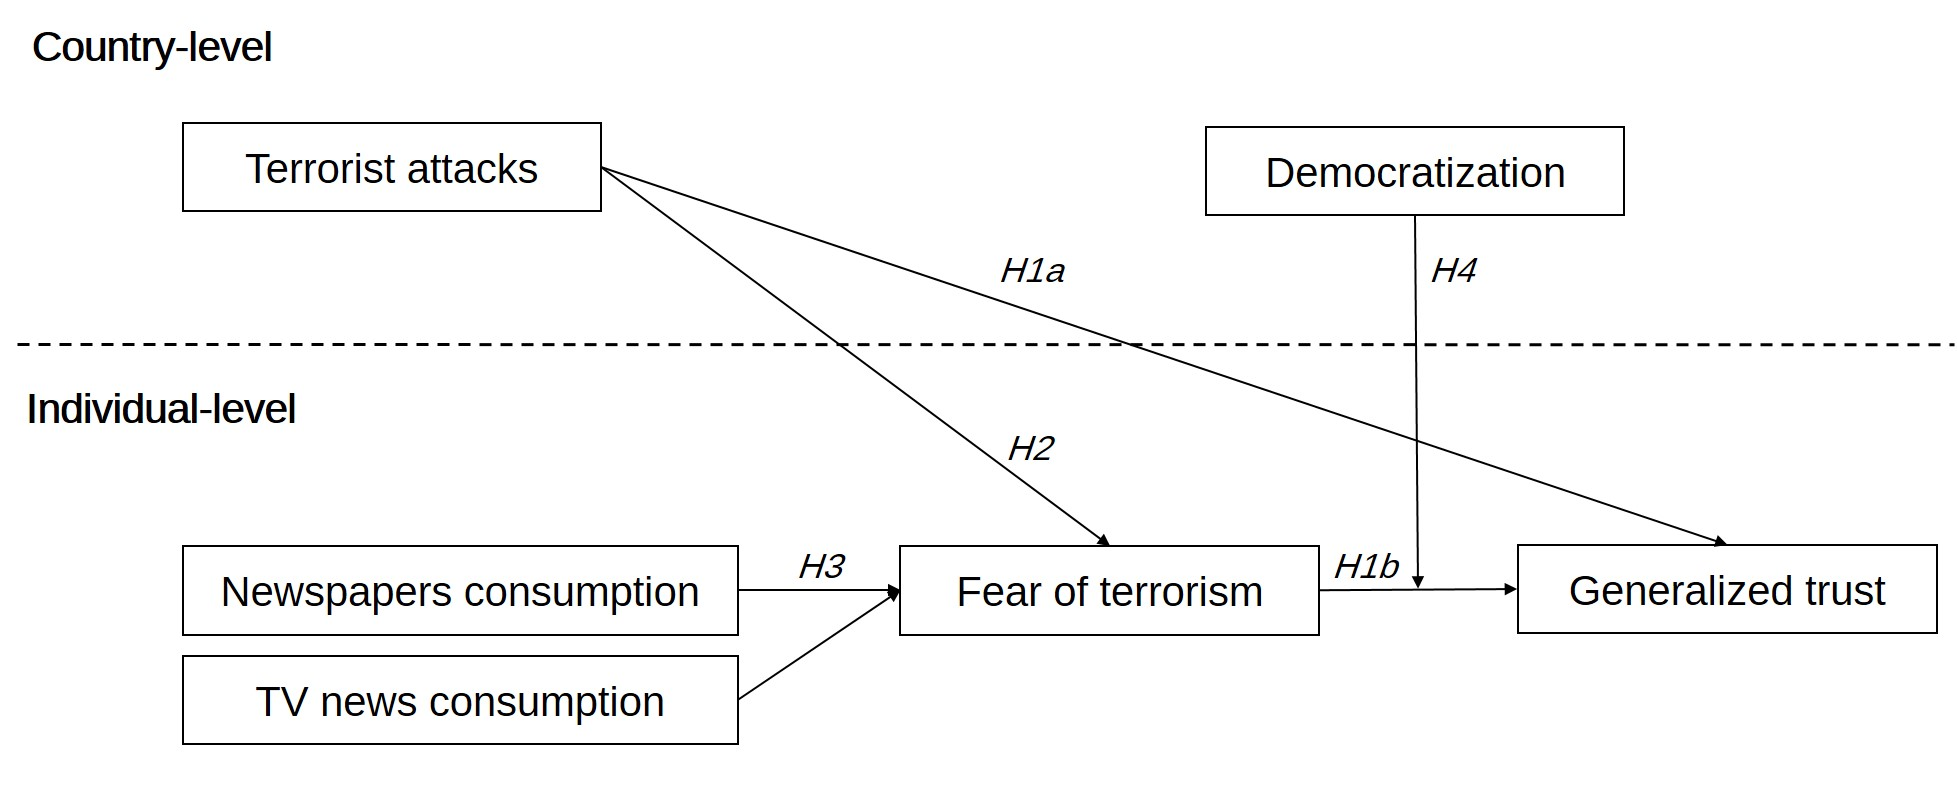
\includegraphics[width=\textwidth]{Chapter_2/art1-model.jpg}}
\caption{Theoretical Model of the Relation Between Terrorism and Trust}
\label{fig:art1-model}    
\end{figure}
%----------------------------------------------------------


%----------------------------------------------------------
\section{Data and Methods}
%----------------------------------------------------------
%----------------------------------------------------------
\subsection{Data}
%----------------------------------------------------------
To understand the impact of terror(ism) on trust, we combine individual-level survey data of the most recent World Values Survey (WVS, Round 6, 2010–2014) with several indicators at the country-level. The WVS carries out face-to-face surveys every five years based on national probability samples with the chance of selection proportionate to population size. After applying list-wise deletion on all indicators included, 76,254 respondents nested within 54 countries are used in this study.\footnote{It is important to note here that several instructive case-studies for the topic under investigation (case-studies often terrorized by homegrown terrorism)---such as Israel, Afghanistan, Syria Somalia, Kenya, or Mali---are not included in the WVS-6 sample and, hence, could not be included in our analyses. Palestine (i.e., respondents from the West Bank and Gaza Strip), on the other hand, was included in the sample, but contained missing values on crucial variables. Since we applied a list-wise deletion technique, respondents from the West Bank and Gaza Strip were dropped from the final sample. Future research could investigate how our proposed model operates within those contexts.} The strength of using WVS is that the sample includes countries from all geographical regions, ranging from developed democracies to developing autocracies. Table \ref{tab:art1-tab1} provides an overview of all countries included, as well as the aggregate measures of our main variables.

%----------------------------------------------------------
% Table 1
%----------------------------------------------------------
\begingroup
\footnotesize
\begin{longtable}[h!]{lC{1.6cm}C{1.6cm}C{1.6cm}cc}
\caption{Trust, Terror, and Terrorism Per Country}
\label{tab:art1-tab1}\\
\hline
Country &
  N &
  \begin{tabular}[c]{@{}c@{}}Trust \% \\ (WVS)\end{tabular} &
  \begin{tabular}[c]{@{}c@{}}Fear \% \\ (WVS)\end{tabular} &
  \begin{tabular}[c]{@{}c@{}}Lethal attacks\\ (GTD)\end{tabular} &
  \begin{tabular}[c]{@{}c@{}}Terrorism index\\ (GTI)\end{tabular} \\ 
\hline
\endfirsthead
%
\multicolumn{6}{c}%
{{Table \thetable\ continued \dots}} \\
\hline
Country &
  N &
  \begin{tabular}[c]{@{}c@{}}Trust \%  \\ (WVS)\end{tabular} &
  \begin{tabular}[c]{@{}c@{}}Fear \%  \\ (WVS)\end{tabular} &
  \begin{tabular}[c]{@{}c@{}}Lethal attacks\\ (GTD)\end{tabular} &
  \begin{tabular}[c]{@{}c@{}}Terrorism index\\ (GTI)\end{tabular} \\ \hline
\endhead
\hline
\multicolumn{6}{r}{\textit{Continued on next page}} \\
\endfoot
\hline
\endlastfoot
%
Algeria             & 1058 & 18.2\% & 78.64\% & 24   & 5.30 \\
Armenia             & 1075 & 10.1\% & 88.28\% & 0    & 1.17 \\
Australia           & 1008 & 57.1\% & 30.95\% & 0    & 1.33 \\
Azerbaijan          & 950  & 16.5\% & 81.89\% & 0    & 2.08 \\
Bahrain             & 1149 & 34.0\% & 35.68\% & 7    & 4.67 \\
Belarus             & 1355 & 35.1\% & 64.94\% & 1    & 2.21 \\
Brazil              & 1429 & 6.2\%  & 66.34\% & 4    & 1.62 \\
Chile               & 926  & 12.9\% & 41.68\% & 0    & 3.48 \\
China               & 1744 & 65.7\% & 47.76\% & 5    & 4.70 \\
Colombia            & 1410 & 4.1\%  & 90.14\% & 75   & 6.32 \\
Cyprus              & 931  & 9.5\%  & 51.45\% & 0    & 0.10 \\
Ecuador             & 1198 & 7.2\%  & 74.21\% & 1    & 1.07 \\
Egypt               & 1467 & 19.6\% & 76.01\% & 13   & 4.88 \\
Estonia             & 1416 & 39.3\% & 47.88\% & 1    & 0.00 \\
Georgia             & 1184 & 9.0\%  & 94.00\% & 1    & 2.95 \\
Germany             & 1971 & 42.7\% & 37.14\% & 0    & 2.48 \\
Ghana               & 1543 & 5.0\%  & 81.98\% & 0    & 0.00 \\
India               & 4580 & 21.3\% & 67.01\% & 483  & 7.95 \\
Iraq                & 1093 & 31.9\% & 80.51\% & 1639 & 9.13 \\
Japan               & 1984 & 39.2\% & 83.87\% & 0    & 2.05 \\
Jordan              & 1195 & 13.3\% & 54.23\% & 1    & 1.96 \\
Kazakhstan          & 1465 & 38.9\% & 77.68\% & 2    & 0.31 \\
Korea, South        & 1092 & 29.9\% & 55.68\% & 0    & 0.03 \\
Kuwait              & 991  & 30.5\% & 66.40\% & 0    & 0.04 \\
Kyrgyzstan          & 1352 & 37.8\% & 79.51\% & 0    & 1.66 \\
Lebanon             & 1020 & 10.9\% & 74.71\% & 24   & 4.48 \\
Libya               & 1859 & 11.0\% & 82.46\% & 146  & 6.32 \\
Malaysia            & 1288 & 8.2\%  & 92.24\% & 0    & 0.32 \\
Mexico              & 1985 & 12.3\% & 86.50\% & 0    & 2.42 \\
Netherlands         & 1753 & 68.9\% & 11.18\% & 0    & 2.36 \\
New Zealand         & 698  & 58.5\% & 22.49\% & 0    & 0.19 \\
Nigeria             & 1733 & 14.6\% & 80.78\% & 38   & 6.31 \\
Pakistan            & 1112 & 24.3\% & 73.92\% & 1102 & 8.67 \\
Peru                & 1153 & 8.1\%  & 84.48\% & 1    & 2.57 \\
Philippines         & 1190 & 2.9\%  & 88.49\% & 156  & 6.77 \\
Poland              & 903  & 22.8\% & 46.07\% & 0    & 0.00 \\
Qatar               & 1046 & 21.2\% & 83.08\% & 0    & 0.20 \\
Romania             & 1393 & 6.2\%  & 61.31\% & 0    & 0.03 \\
Russia              & 2197 & 28.8\% & 80.15\% & 169  & 7.00 \\
Rwanda              & 1523 & 16.6\% & 97.11\% & 3    & 3.66 \\
Singapore           & 1843 & 39.1\% & 46.34\% & 0    & 0.00 \\
Slovenia            & 1016 & 20.3\% & 35.04\% & 0    & 0.00 \\
South Africa        & 3199 & 24.2\% & 49.92\% & 5    & 2.52 \\
Sweden              & 1132 & 65.5\% & 22.53\% & 1    & 2.56 \\
Thailand            & 1060 & 31.8\% & 58.21\% & 242  & 7.07 \\
Trinidad \& Tobago  & 978  & 3.2\%  & 44.68\% & 0    & 0.09 \\
Tunisia             & 1133 & 16.1\% & 97.88\% & 8    & 2.05 \\
Turkey              & 1475 & 12.1\% & 70.92\% & 25   & 5.22 \\
Ukraine             & 1350 & 25.2\% & 64.96\% & 1    & 2.57 \\
United States       & 2137 & 38.4\% & 53.58\% & 6    & 4.33 \\
Uruguay             & 850  & 14.4\% & 49.53\% & 0    & 0.00 \\
Uzbekistan          & 1349 & 14.5\% & 47.07\% & 0    & 1.93 \\
Yemen               & 874  & 40.5\% & 92.91\% & 348  & 7.16 \\
Zimbabwe            & 1439 & 6.4\%  & 62.96\% & 1    & 1.51 \\
\textit{Total} &
  \textit{77409} &
  \textit{24.59\%} &
  \textit{65.38\%} &
  \textit{4533} &
  \textit{3.16} \\ \hline
\end{longtable}
\endgroup

%----------------------------------------------------------
\subsection{Measurements}
%----------------------------------------------------------

\subsubsection{Dependent Variable: Generalized Trust}
As to the dependent variable, we rely on the well-known notion of generalized trust or trust towards strangers. Generalized trust in the WVS is measured using the question: ``In general, do you think most people can be trusted (=1), or that you can’t be too careful in dealing with other people (=0)?'' Although this often criticized dichotomous measure does not allow much detail in the measurement of the latent attitude ``trust'' \citep[e.g.,][]{Lundmark2016}, there is ample counter-evidence that the question is a relatively valid and reliable measure of the underlying theoretical construct of `trustworthiness' as it has shown measurement equivalence, strong test-retest stability, and concurrent validity.\footnote{\cite{Knack1997}, for instance, validated the standard question by showing significant correlations between the proportion of people who said that most people can be trusted and the proportion of people who returned intentionally lost wallets. In other words, the mean national response on the trust question highly corresponds with real-life trustworthy behavior, which reflects the conclusion of Glaeser and colleagues \citeyear{Glaeser2000} based on various experiments. See also \cite{Delhey2005a} or \cite{Uslaner2012}.}


An important feature for our multilevel setting is that there is a substantial degree of variation in trust across the countries included. Table \ref{tab:art1-tab1} shows that this is indeed the case. The aggregated percentage of trusting individuals in a country ranges from a mere 2.9 percent in the Philippines to 68.9 percent in the Netherlands. More specifically, an empty random intercepts model indicates that 24.2 percent of the variance lies at the country level. In other words, generalized trust systematically varies across countries, making it methodologically necessary to model these contextual differences \citep{Hox2010}.


\subsubsection{Independent Variables}
\textbf{\textit{Terrorist Attacks.}} To capture county-level exposure to terrorism, we use the Global Terrorism Index (GTI). The GTI provides a broad measure of the impact of terrorist attacks as it ranks countries based on four indicators (i.e., number of attacks, fatalities, wounded, and property damage) weighted over five years.\footnote{For more information on operationalization, please see \cite{TheInstituteforEconomicsandPeace2016}.} As a robustness check of the model, we also include the number of fatal attacks that occurred within a two-year period prior to the starting month of the survey. Only attacks that resulted in at least one fatality are considered to capture incidences that are most salient to the population, and we lagged the variable to ensure that the models capture trust levels after the violent incidences. To construct this rude indicator of terrorist activity, we relied on incidence count data from the Global Terrorism Database (GTD). Attacks included in GTD need to be conducted by sub-national actors outside the context of legitimate warfare activities and, hence, differentiate from civil wars, internal armed conflict, and state terrorism. Because this variable is heavily skewed to zero, we also use a dichotomous variable indicating whether a country has witnessed at least one fatal attack in the last two years or not.


\vspace{3mm}
\noindent\textbf{\textit{News Exposure.}} Television news consumption and newspaper consumption is measured by asking respondents the following question: ``People learn what is going on in this country and the world from various sources. For each of the following sources, please indicate whether you use it to obtain information daily, weekly, monthly, less than monthly or never: [Daily newspaper; TV news].'' Due to data limitations, we cannot include a more fine-grained measure of terrorism-related news exposure. Importantly, the bivariate correlation between newspaper and television news consumption is remarkably low ($r = .241$, $p < .001$) and the Variance Inflation Factor shows no problem with multicollinearity when including both variables simultaneously in the models.


\subsubsection{Mediator and Moderator}
\noindent\textbf{\textit{Fear of Terrorism.}} To operationalize fear of terrorism, we tap into the psychological trauma caused by terrorism; that is the extent to which an individual is worried about terror attacks \citep{Sinclair2012}. One of the main advantages of the WVS is that the survey asks about how worried people are about future terror attacks. The original four-point scale is dichotomized for practical reasons, distinguishing people who are not (much) worried about terror attacks (=0) from people who are (much) worried about terror attacks (=1). Again, Table \ref{tab:art1-tab1} shows that there is a substantial degree of variation in fearing terrorist attacks across the countries included. The aggregated percentage of afraid individuals in a country ranges from 11.7 percent in the Netherlands to 97.1 percent in Rwanda. An empty random intercepts model indicates that a remarkable 29.0 percent of the variance lies at the country level.

\vspace{3mm}
\noindent\textbf{\textit{Democratization.}} As a measure of the level of democracy in a country, the Freedom House/Imputed PolityIV of the Quality of Government Database is included. This variable uses a comprehensive definition of democracy and takes into account qualitative aspects such as political rights and civil liberties (Freedom House) as well as constraints on the executive (Polity IV). This average index is found to perform better both in terms of validity and reliability than its constituent parts. Zero signifies the least democratic score, while ten is most democratic.\footnote{The exact construction of this index is detailed as follows: ``[S]cale ranges from 0–10 where 0 is least democratic and 10 most democratic. Average of Freedom House (fh\_pr and fh\_cl) is transformed to a scale 0–10 and Polity (p\_polity2) is transformed to a scale 0–10. These variables are averaged into fh\_polity2. The imputed version has imputed values for countries where data on Polity is missing by regressing Polity on the average Freedom House measure. \cite{Hadenius2005} show that this average index performs better both in terms of validity and reliability than its constituent parts.''}


\subsubsection{Control Variables}
We attempt to alleviate concerns of omitted or confounding variables by including several control variables previously linked to trust or terror. As individual-level controls, we include measures of age (in years), gender (0 = female, 1 = male), education (0–8), employment status (0 = employed, 1 = unemployed), and political interest (0–3). As country-level controls, we include measures of wealth (ln\_GDP) and income inequality (Gini coefficient) in addition to the level of democracy. The country-level variables were lagged with one year before the start-year of the WVS. Appendix \ref{app:B1} summarizes the descriptive statistics of the controls. 


%----------------------------------------------------------
\subsection{Method}
%----------------------------------------------------------

Our theoretical model predicts direct, indirect, and moderated relations between terror(ism), generalized trust, news exposure, and democratization. Additionally, our data-structure is inherently hierarchical since individuals are nested within their countries. Hence, we conduct multilevel\footnote{A multilevel approach enables us to examine individual- and country-level predictors simultaneously, while also correctly taking into account the clustering of our respondents within their countries. For more information, see \cite{Gelman2007} or \cite{Hox2010}.} path analyses\footnote{A structural equation approach enables us to hypothesize and test our chain of (causal) relations between the variables by estimating multiple structural (i.e., regression) equations simultaneously. For more information, see \cite{Kline2015}.} in Mplus 8 \citep{Muthen2015}. A maximum likelihood estimator with robust standard errors using a numerical integration algorithm is used. This estimator, using a Monte Carlo integration, is robust to non-normality and can be used for categorical/dichotomous variables \citep{Muthen2015}. Furthermore, because of inherent difficulties with centering in ML-SEM, reported coefficients are uncentered in the multilevel path models.\footnote{Centering level-1 predictors considerably changes the relationships between variables, as some predictors are, in turn, also outcomes. For more information, see \cite{CastanhoSilva2019}.} Last, although path models suggest directionality, the cross-sectional nature of our analyses cannot guarantee the absence of reversed causality in the hypothesized relationship nor do we test the presence of other relationships between the concepts included in Figure \ref{fig:art1-model}.

In the following sections, after presenting the relevant bivariate correlations, we analyze how terrorist attacks as well as the fear of future attacks are related to social trust among citizens in 54 countries (H1-2), and we assess the role of the media in exacerbating this relationship (H3). Building on the theories of community resilience, we lastly examine differences in the relationship between fear and trust across countries with a special focus on the moderating role of democratization (H4).


%----------------------------------------------------------
\section{Results}
%----------------------------------------------------------
%----------------------------------------------------------
\subsection{Bivariate Correlations}
%----------------------------------------------------------
As a first step of testing our theoretical model, we examine the bivariate correlations between the variables. Our model suggests a causal chain in which direct and indirect exposure to terror attacks induce fear of terrorism, which in turn decreases trust. Since the model largely relies on the assumption that terrorism and fearing terrorism are two distinct concepts both influencing trust, we first present a simple correlation between the percentages of fear in a country and the objective threat of terrorism in that country (including both the GTI of a country and the number of lethal terror attacks in that country; see, respectively, Figure \ref{fig:art1-corr1} and \ref{fig:art1-corr2} on the next pages). 


In keeping with previous studies on the association between real-life crime rates and fear of crime, the correlation between the number of lethal attacks in a country and the proportion of citizens that fear terrorism is rather weak and insignificant ($r = .180$, $p = .194$). The correlation between aggregated fear percentages and the GTI just reaches significance ($r = .311$, $p = .022$). Hence, both terrorism and fearing future terrorism will still be included as separate predictors of trust in our path models below. Interestingly, generalized trust is uncorrelated with either terror attacks ($r = .005$, $p = .971$) or the GTI ($r = .049$, $p = .724$). In contrast, fearing terrorism is negatively and highly significantly correlated to trust ($\phi = -.135$, $p < .001$). It is noteworthy here that both levels of fear and distrust are very high. Overall, a mere 24.6 percent of the respondents report that most people can be trusted, while 75.4 percent of the people think that you cannot be too careful when dealing with other people. Likewise, only 34.6 percent of the respondents indicate not to worry about future terror attacks in his/her country, while 65.4 percent of the respondents worry about such attacks. Remarkably, while fear is positively correlated with TV news consumption ($r_{pb} = .041$, $p < .001$), newspaper consumption is negatively associated with fear of terrorism ($r_{pb} = -.078$, $p < .001$).

In sum, bivariate correlations among the variables of interest are generally consistent with our hypotheses with the notable exception of the insignificant relation between the objective threat of terrorism and trust. However, these are single bivariate correlations based on the full sample (N = 76,254) or on the country sample (N = 54) and, hence, ignore the inherent hierarchy of the data as well as the hypothesized causal chains.

%----------------------------------------------------------
% Figure 2: Correlations 1
%----------------------------------------------------------
\begin{sidewaysfigure}[!]
    \fbox{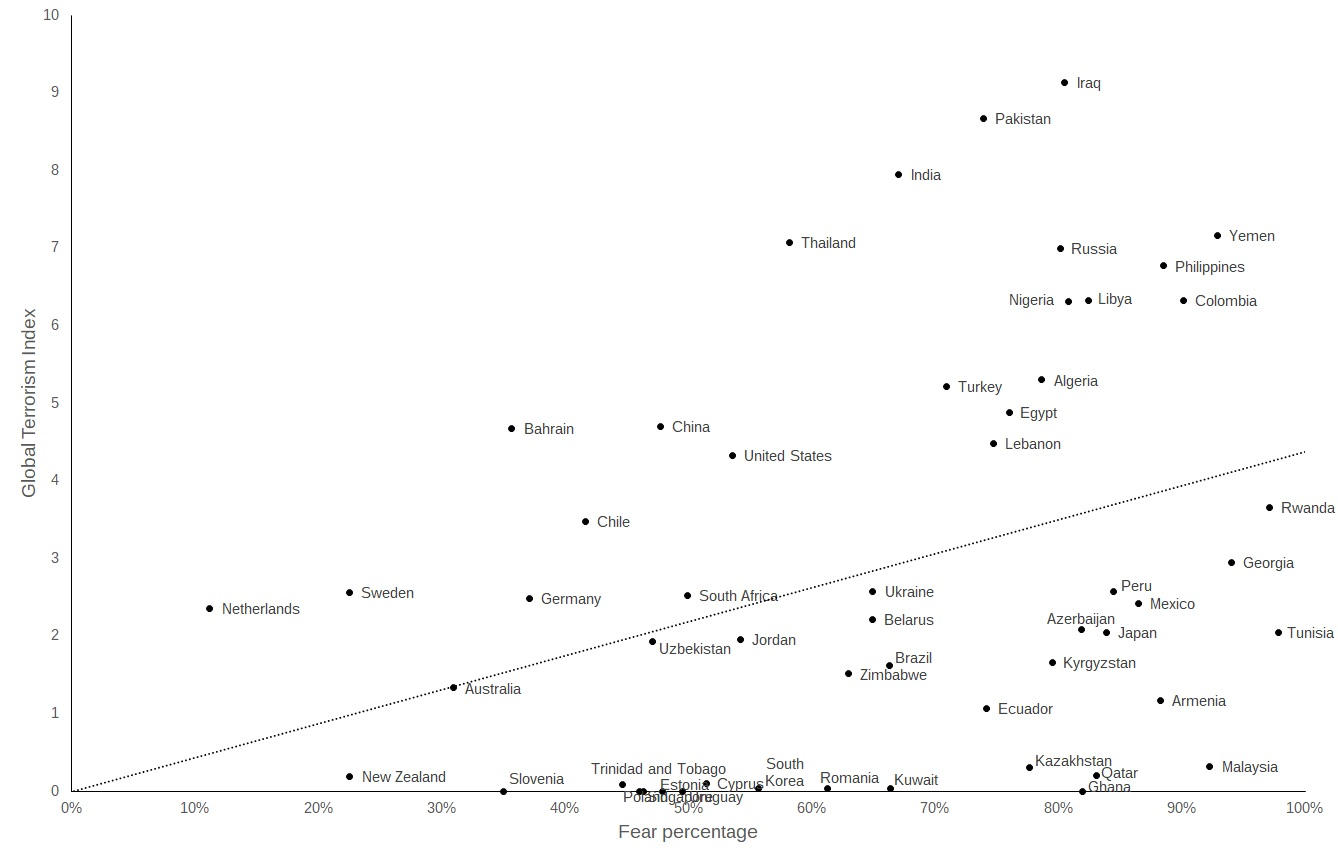
\includegraphics[width=\textwidth]{Chapter_2/art1-corr1.jpg}}
    \caption{Relation Between Fearing Terrorism and Global Terrorism Index}
    \label{fig:art1-corr1}
\end{sidewaysfigure}

%----------------------------------------------------------
% Figure 3: Correlations 2
%----------------------------------------------------------
\begin{sidewaysfigure}[!]
    \fbox{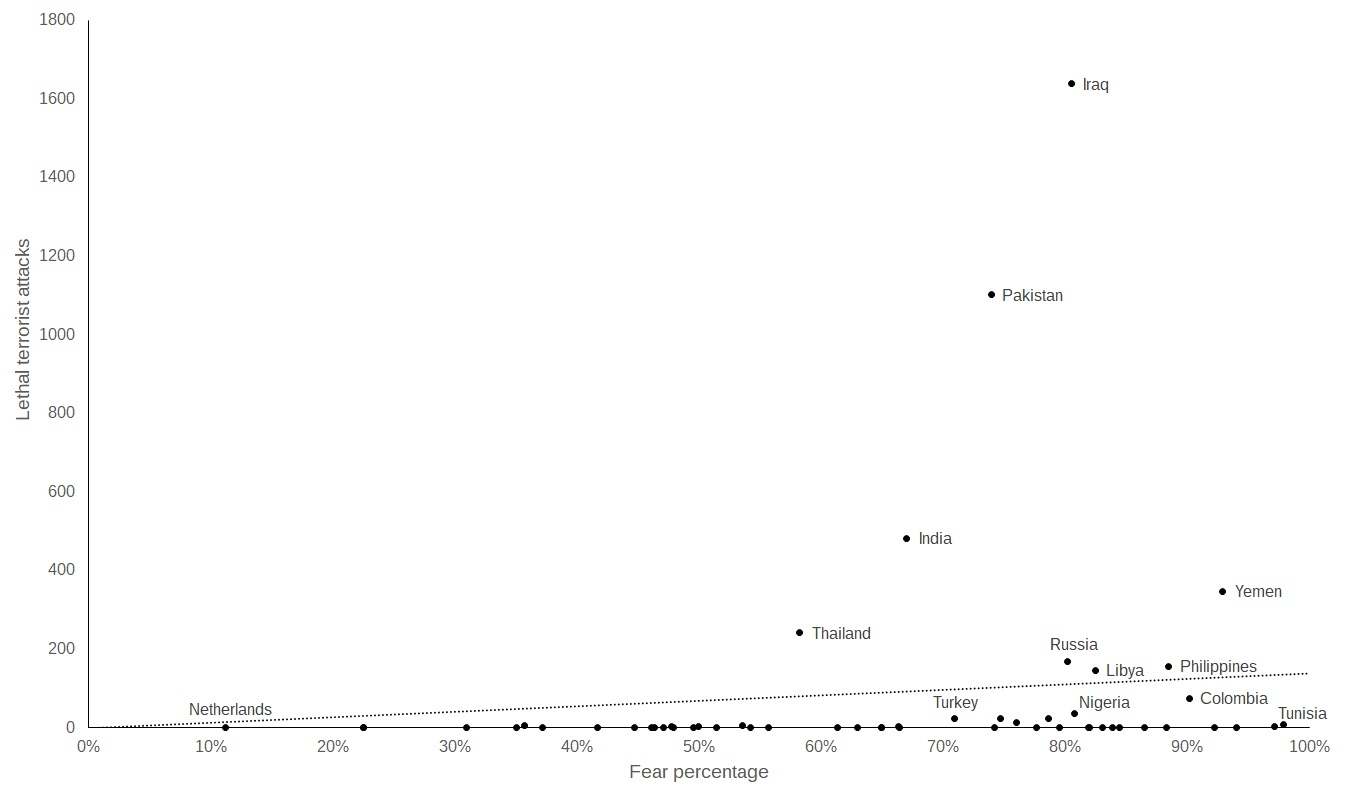
\includegraphics[width=\textwidth]{Chapter_2/art1-corr2.jpg}}
    \caption{Relation Between Fearing Terrorism and Lethal Terrorist Attacks}
    \label{fig:art1-corr2}
\end{sidewaysfigure}
%----------------------------------------------------------


%----------------------------------------------------------
\newpage
\subsection{Multilevel Path Model}
%----------------------------------------------------------
Next, we advance with the multilevel path model based upon the hypothesized relations. Direct and indirect exposure to the objective threat of terrorism are assessed as exogenous variables, fearing terrorism as a mediating variable, and generalized trust as the dependent one. Figure \ref{fig:art1-results1} displays these direct and indirect relations between the variables of interest, while controlling for other individual- and country-level characteristics. In contrast with the expectations and bivariate correlations, the objective impact of terrorist attacks on a country has a positive association with generalized trust ($b = .063$, $p < .001$)---after accounting for the fear of terrorism and other individual- and country-level variables. These results do not change when we re-estimate the model using the dichotomous attack variable ($b = .165$, $p < .05$). Fearing terrorism, on the other hand, significantly decreases the likelihood of generalized trust ($b = -.252$, $p < .001$). More specifically, respondents who fear terrorism are about 4.37 percent less likely to trust others compared to respondents who do not fear future attacks. In other words, H1 is partially confirmed: Subjective threat perceptions decrease social trust (i.e., H1b confirmed) over and above the objective terror threat (i.e., H1a refuted). 

%----------------------------------------------------------
% Figure 4: Path model results
%----------------------------------------------------------
\begin{figure}[H]
\centering
\fbox{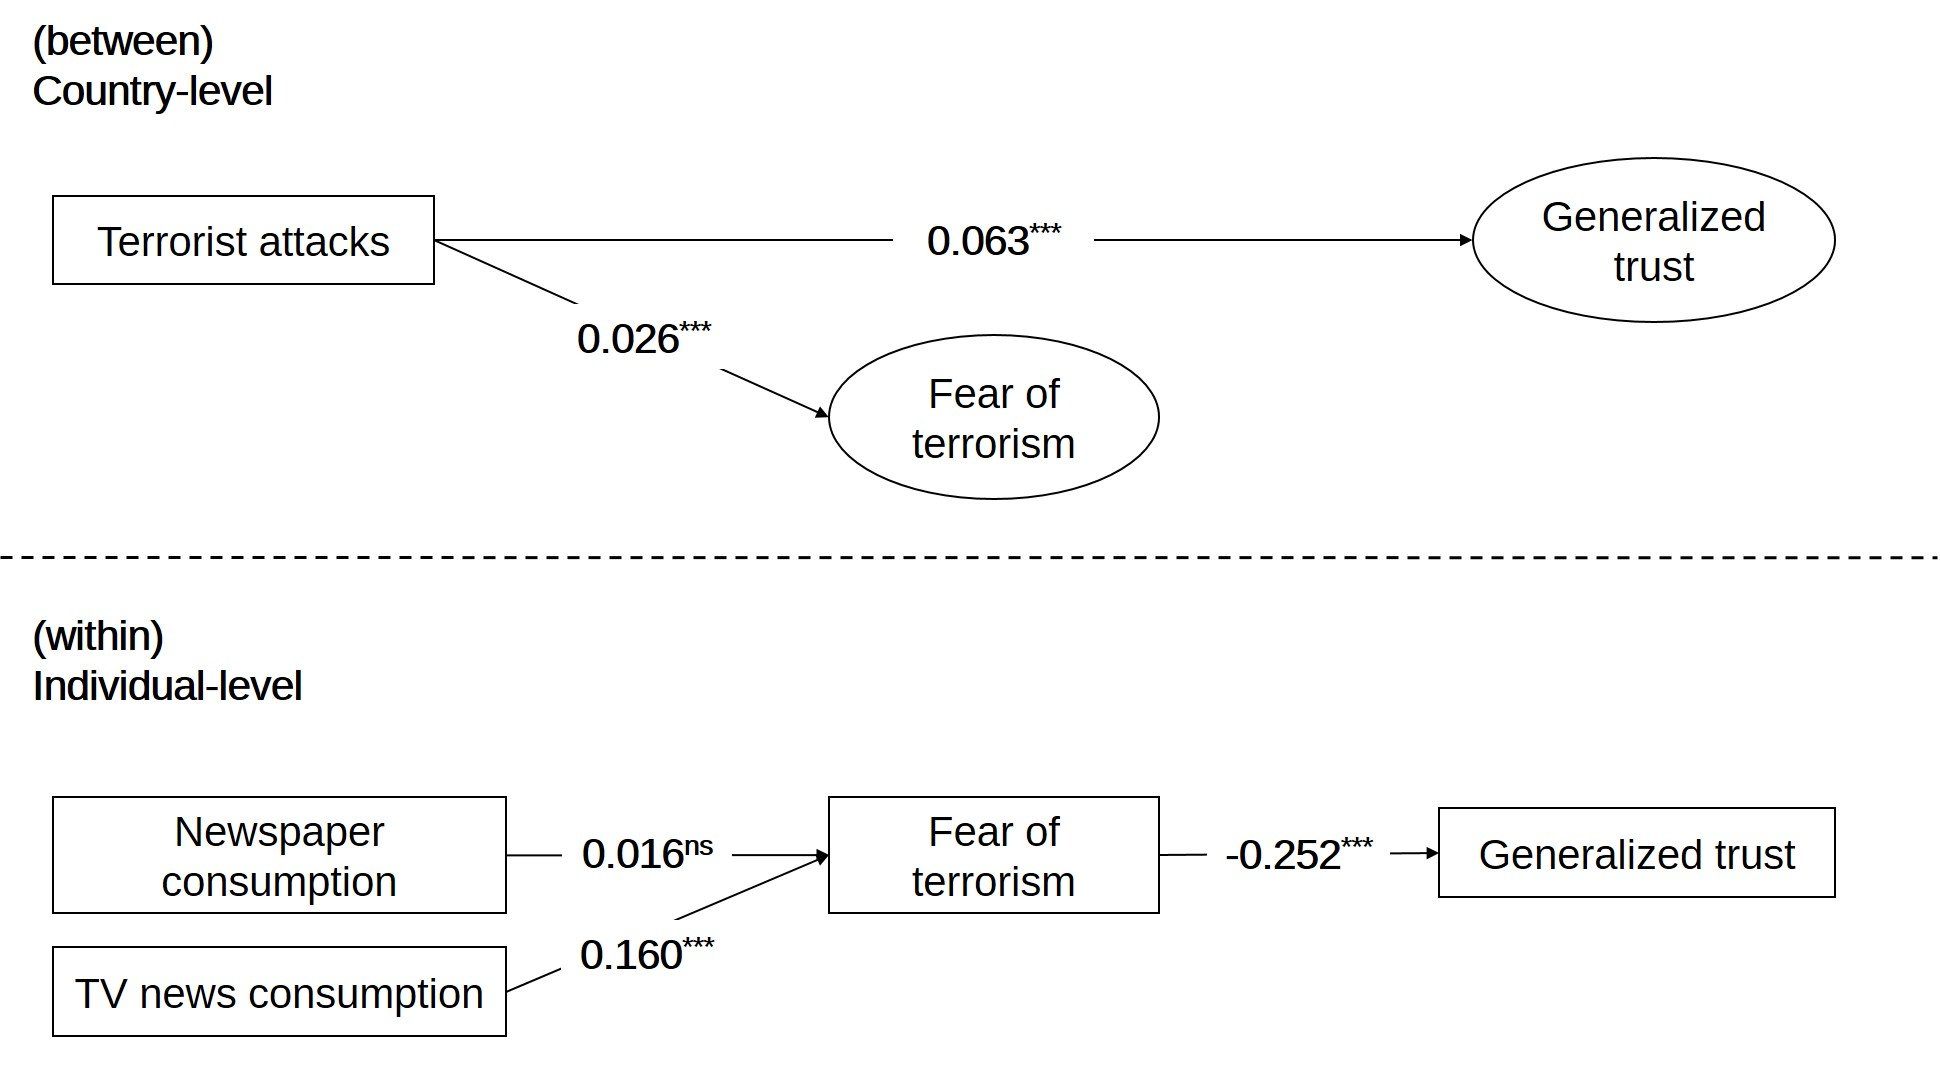
\includegraphics[width=0.98\textwidth]{Chapter_2/art1-results1.jpg}}
\caption{Random Intercepts Path Model}
\label{fig:art1-results1}    
\end{figure}
%----------------------------------------------------------

Terrorism still affects social trust indirectly (and negatively) by increasing the probabilities that people fear terrorism ($b = .026$, $p < .001$), confirming H2. Likewise, citizens of countries that have suffered at least one lethal attack prior to the survey are more likely to fear terrorism ($b = .299$, $p < .001$). In addition to such direct exposure to attacks, possible indirect exposure through news consumption also increases fear, albeit only via television news consumption ($b = .160$, $p < .001$). Hence, H3 is also (partially) confirmed.


Furthermore, as to the individual-level determinants of social trust, watching television news decreases the likelihood of trust ($b = -.071$, $p < .001$), while reading newspapers does not significantly increase its likelihood ($b = .029$, $p = .093$). The higher educated and the more politically interested respondents are also more likely to trust strangers ($b = .061$, $p < .001$ for education; and $b = .096, p < .001$ for political interest), while unemployment is negatively but not significantly associated with trust ($b = -.060$, $p = .113$). Age and trust are positively associated ($b = .004$, $p < .01$), but gender is not significantly related to trust ($b = .014$, $p = .617$). As to the country-level control variables, economic wealth increases the likelihood of generalized trust ($b = .067$, $p < .001$), while an unequal distribution of that wealth decreases the likelihood of generalized trust ($b = -.031$, $p < .001$). Last, democratization is negatively associated with trust ($b = -.074$, $p < .001$).


As to the individual-level determinants of fearing terrorism, men are less likely to fear future terrorist attacks ($b = -.160$, $p < .001$), while higher educated respondents are less likely to fear attacks ($b = -.023$, $p < .05$). Political interest and fear are also positively associated ($b = .075$, $p < .01$), whereas age and unemployment are not significantly impacting the odds of fear ($b = .001$, $p = .428$ for age; and $b = .054$, $p = .108$ for unemployment). As to the country-level determinants of fearing terrorism, citizens in less wealthy, more unequal, and less democratic countries are more likely to be afraid of future terrorist attacks ($b = -.150$, $p < .001$ for GDP; $b = .021$, $p < .001$ for Gini; and $b = -.094$, $p < .001$ for PolityIV).



%----------------------------------------------------------
\subsection{Multilevel Regression Models}
%----------------------------------------------------------

The model presented in Figure \ref{fig:art1-results1} produced some interesting findings regarding the relationships between terrorism, fearing terrorism, and trust. Nevertheless, we contend that there is yet more to discover by assuming that the effect of fear on trust is not univocal across countries. Indeed, when breaking down the relationship between fear and trust on a country-by-country basis, we find heterogeneity in the effect of fear on trust. While the effect of fear is generally negative, it clearly has a varying strength with some positive slopes in, for instance, Iraq (1.06) and Thailand (0.70). As a result of this, in our final model we allow this relationship to (randomly) vary across countries, and we specifically assess the role of democratization as a possible predictor of this variance. In more statistical words, we include a random slope and democratization is considered a potential moderator for the slope of fear tested via a cross-level interaction effect between fear and democratization. We study this last hypothesis by means of a multilevel regression analysis in R instead of our path model because introducing a random slope and cross-level interaction effect combined with a dichotomous dependent and mediating variable is too computationally demanding in the currently (i.e., summer 2018) available statistical software. Moreover, a multilevel framework offers more opportunities to scrutinize variances in slopes and intercepts. Last, as the fourth hypothesis only concerns the last link in our theoretical model, a standard regression analysis is also adequate.


Hence, in these final analyses, generalized trust constitutes the dependent variables and fear of terrorism the key independent variable. We again control for the same individual and country-level characteristics as above. Table \ref{tab:art1-tab2} includes various multilevel regression models. Firstly, Model 1 in Table \ref{tab:art1-tab2} demonstrates that the effects of the individual- and country-level characteristics largely correspond to the results of the multilevel path model above. More importantly, the variance of our slope is significant. Following our model, we argue that the impact of fearing terrorism on citizens’ generalized trust will vary between countries depending on the level of democratization in countries. This cross-level interaction effect between fear and democratization is indeed negatively significant ($b = -.044$, $p < .05$). Hence, the likelihood of trust is more negatively affected by people’s concerns with terrorist attacks in more democratic societies. Figure \ref{fig:art1-results2} aids to interpret this cross-level interaction effect. As you can see, when the democratization indicator increases (hence, in more democratic countries), the effect of fearing terrorism on trust becomes more negative. In contrast, in the least democratic countries, fearing terrorism does not significantly impact trust, which corresponds to the coefficient of fear ($b = .03$, $p = .77$) in Model 2. Accordingly, the last hypothesis is also supported by the empirical evidence. 


Interestingly, and in line with this result, a cross-level interaction between fear and the GTI (see Model 3 in Table \ref{tab:art1-tab2}) also shows that the effect of fear on trust is stronger in these countries where terrorism remains a rather imagined danger ($b = .041$, $p = .055$; see right panel in Figure \ref{fig:art1-results2}). Or, when terrorism constitutes part of one’s daily routine, the fear of future attacks does not significantly impact trust anymore. However, this cross-level interaction fails to meet the critical value of significance ($p = .05$), and, hence, the model including this interaction is no significant improvement ($\chi^2 = 3.48$, $p = .06$).


%----------------------------------------------------------
% Table 2
%----------------------------------------------------------
\vspace{3mm}
\begin{table}[H]
\caption{Conditional Effect of Fearing Terrorism on Trust}
\label{tab:art1-tab2}
\onehalfspacing
\resizebox{\textwidth}{!}{%
\begin{tabular}{llccc}
\hline
\multicolumn{2}{l}{\begin{tabular}[c]{@{}c@{}} \\ \\ Parameter\end{tabular}} &
  \begin{tabular}[c]{@{}c@{}}Model 1: \\ random\\ intercept model\end{tabular} &
  \begin{tabular}[c]{@{}c@{}}Model 2: \\ random slopes \\ model (democratization)\end{tabular} &
  \begin{tabular}[c]{@{}c@{}}Model 3:\\ random slopes \\ model (GTI)\end{tabular} \\ \hline
\multicolumn{2}{l}{}                        & \multicolumn{3}{c}{Fixed effects}                   \\ \cline{3-5} 
\multicolumn{2}{l}{Intercept}               & $-3.00$ (1.09)\textsuperscript{**}   & $-3.21$ (0.96)\textsuperscript{***}  & $-2.89$ (1.06)\textsuperscript{**}   \\
\multicolumn{2}{l}{Level 1: Individuals}    &                 &                 &                 \\
            & Fearing terrorism             & $-0.25$ (0.02)\textsuperscript{***}  & 0.03 (0.77)     & $-0.37$ (0.08)\textsuperscript{***}  \\
            & Gender (ref.=Female)          & 0.01 (0.02)     & 0.01 (0.02)     & 0.01 (0.02)     \\
            & Age                           & 0.00 (0.00)\textsuperscript{***}   & 0.00 (0.00)\textsuperscript{***}   & 0.00 (0.00)\textsuperscript{***}   \\
            & Education                     & 0.06 (0.00)\textsuperscript{***}   & 0.06 (0.00)\textsuperscript{***}   & 0.06 (0.00)\textsuperscript{***}   \\
            & Unemployed                    & $-0.06$ (0.02)\textsuperscript{**}   & $-0.05$ (0.02)\textsuperscript{**}   & $-0.05$ (0.02)\textsuperscript{**}   \\
            & Political interest            & 0.10 (0.01)\textsuperscript{***}   & 0.09 (0.01)\textsuperscript{***}   & 0.09 (0.01)\textsuperscript{***}   \\
            & TV news consumption           & $-0.07$ (0.01)\textsuperscript{***}  & $-0.07$ (0.01)\textsuperscript{***}  & $-0.07$ (0.01)\textsuperscript{***}  \\
            & Newspaper consumption         & 0.03 (0.01)\textsuperscript{***}   & 0.03 (0.01)\textsuperscript{***}   & 0.03 (0.01)\textsuperscript{***}   \\
\multicolumn{2}{l}{Level 2: Countries}      &                 &                 &                 \\
            & GTI                           & 0.09 (0.04)\textsuperscript{*}     & 0.10 (0.04)\textsuperscript{*}     & 0.07 (0.05)     \\
            & (ln)GDP                       & 0.38 (0.10)\textsuperscript{***}   & 0.37 (0.09)\textsuperscript{***}   & 0.37 (0.10)\textsuperscript{***}   \\
            & Gini                          & $-0.05$ (0.01)\textsuperscript{***}  & $-0.05$ (0.01)\textsuperscript{***}  & $-0.05$ (0.01)\textsuperscript{***}  \\
            & PolityIV                      & $-0.08$ (0.04)\textsuperscript{*}    & $-0.05$ (0.04)    & $-0.08$ (0.04)\textsuperscript{*}    \\
\multicolumn{2}{l}{Cross-level interaction} &                 &                 &                 \\
            & Fear*PolityIV                 &                 & $-0.04$ (0.02)\textsuperscript{*}    &                 \\
            & Fear*GTI                      &                 &                 & 0.04 (0.02)\textsuperscript{0.05}  \\ \cline{3-5} 
\multicolumn{2}{l}{}                        & \multicolumn{3}{c}{Random effects}                  \\ \cline{3-5} 
\multicolumn{2}{l}{Variance (Intercept)}    & 0.58            & 0.61            & 0.62            \\
\multicolumn{2}{l}{Variance (Fear)}         &                 & 0.12            & 0.13            \\
\multicolumn{2}{l}{Covariance}              &                 & $-0.09$           & $-0.10$           \\
\multicolumn{2}{l}{AIC}                     & 73501.34        & 73345.53        & 73347.93        \\
\multicolumn{2}{l}{BIC}                     & 73630.73        & 73502.64        & 73505.04        \\
\multicolumn{2}{l}{Log Likelihood}          & $-36736.67$       & $-36655.77$       & $-36656.96$       \\ \hline
\end{tabular}%
}
\vspace{-5mm}
\singlespacing
\footnotesize{\textit{Note:} Entries are unstandardized, uncentered maximum likelihood estimations using logistic multilevel models in R. Therefore, and as a result of rounding, some entries are displayed as zero (which they are not). N$_{countries}$ = 54, N$_{individuals}$ = 76,254. AIC = Akaike information criterion, BIC = Bayesian information criterion. \textsuperscript{*}\(p<0.05\), \textsuperscript{**}\(p<0.01\), \textsuperscript{***}\(p<0.001\).}\par
\end{table}
\newpage


%----------------------------------------------------------
% Figure 4: Path model results
%----------------------------------------------------------
\vspace{3mm}
\begin{figure}[h!]
\centering
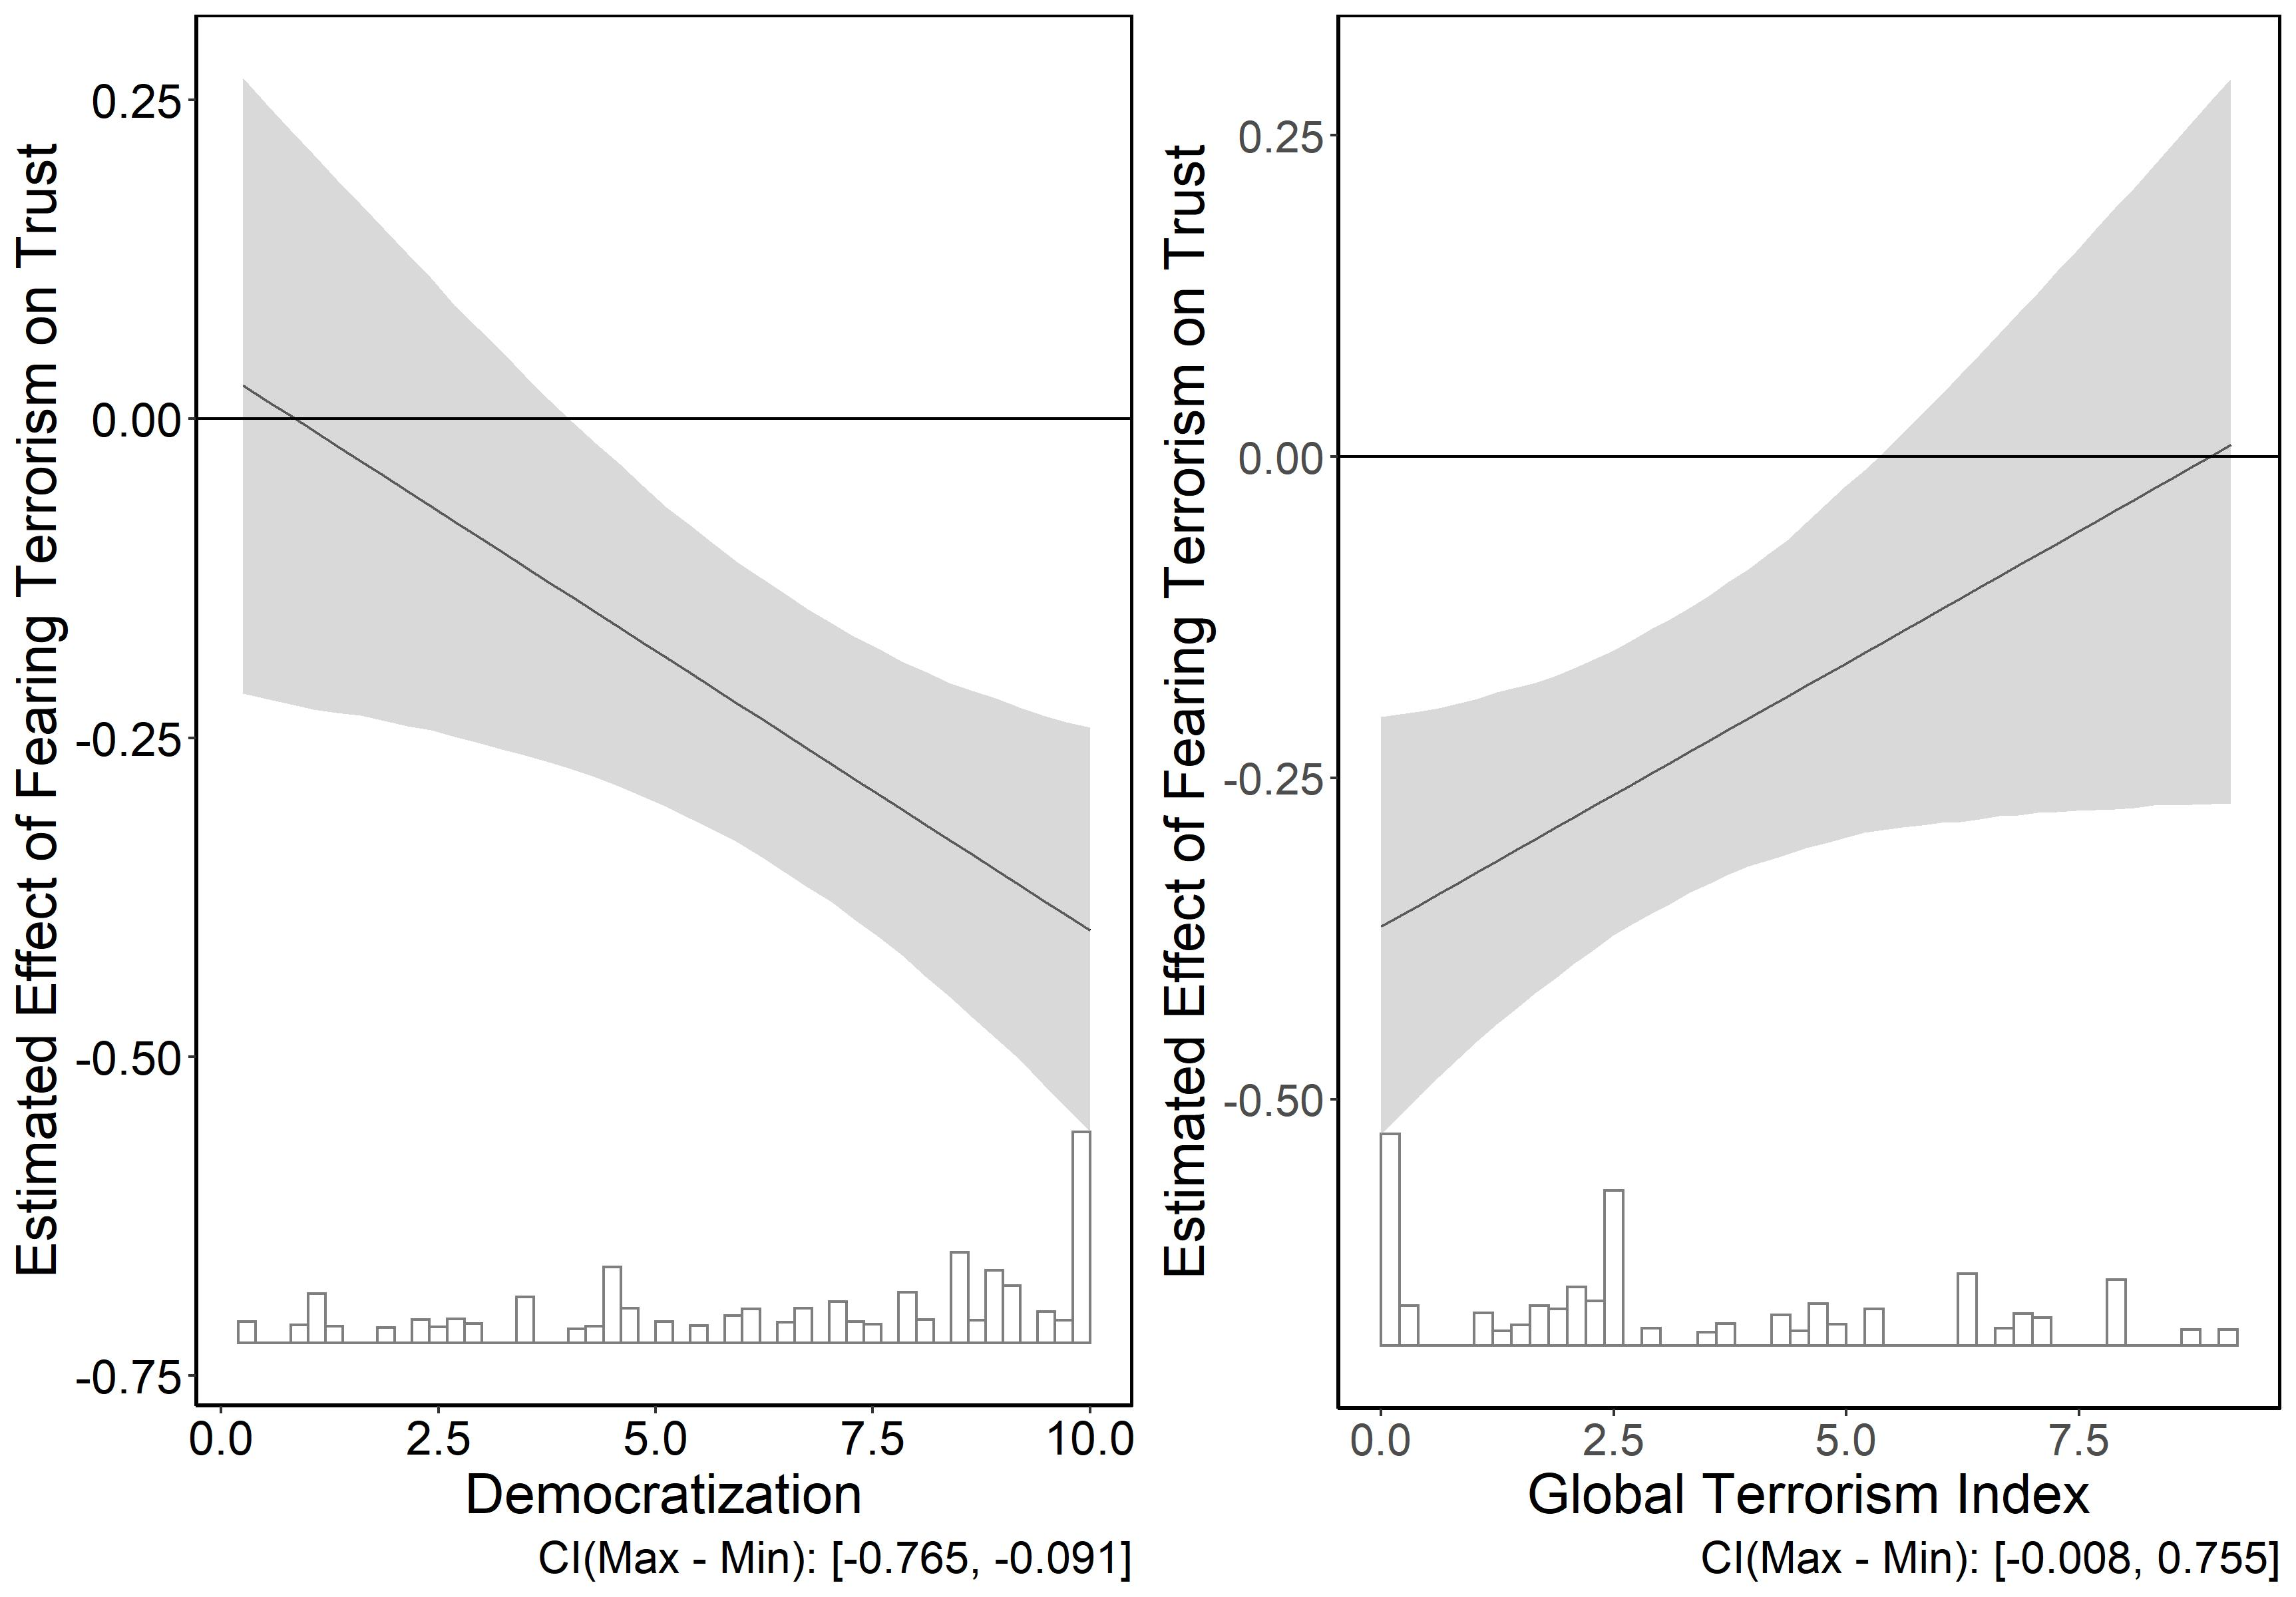
\includegraphics[width=0.98\textwidth]{Chapter_2/art1-results2.jpeg}
\caption{Moderating Effect of Democratization (Left) and GTI (Right) on the Effect of Fearing Terrorism on Trust}
\label{fig:art1-results2}    
\end{figure}
\vspace{3mm}
%----------------------------------------------------------

Before discussing the implications of these findings, we run one more additional robustness check. The reported coefficients were, up until now, uncentered and unstandardized. However, to fully take into account country-specific idiosyncrasies, we re-run the random slope model using group-mean centered level-1 estimates. Group-mean centering takes into account the relative position of a citizen within his country by subtracting individuals’ values on the predictors from the national average. Group-mean centered scores are uncorrelated with country-level variables (i.e., all between-country variation in a variable is erased) and, hence, yields a pure estimate of the pooled within-cluster (i.e., countries) regression coefficients. Therefore, the estimated effect on a level-1 outcome and the interpretation of the coefficients changes substantially. All that is preserved now are relative positions of citizens inside their own country \citep{Enders2007, CastanhoSilva2019}.\footnote{Level-2 estimates are grand mean centered and represent a change from the mean across all countries.} For instance, although people in Rwanda are substantially more afraid of terrorism compared to people in the Netherlands, only the relative differences between individuals within the countries are taken into the model after group-mean centering. This produces a pure estimate of the effect of fear on trust, disregarding all dynamics between countries. The group-mean centered models produce the same results as before (see Appendix \ref{app:B2}). Again, fear of terrorism is negatively associated with social trust while the effect of terrorist attacks now fails to reach significance. The moderation effect of democratization also holds.


%----------------------------------------------------------
\section{Conclusion}
%----------------------------------------------------------

The objective of this chapter was to analyze how terrorism affects social trust across individuals and societies. Trust has long been recognized as a powerful indicator of how cohesive a society is and is often referred to as the ``glue'' that binds people together within a particular society. This ``glue'' seems crucial for the development and functioning of states. In societies with low levels of trust, economic progress is often slower, (political) institutions usually do not function as efficiently and effectively, and general well-being is regularly lower compared to high-trust societies. Despite the importance of trust for the well-functioning of societies, relatively little is known about the relationship among terrorist attacks, fear of terrorism, and the destruction of social trust. While some authors have argued that trust is a fairly stable societal characteristic rather immune to negative experiences \citep{Bauer2015, Jones1996, Uslaner2002, Uslaner2008}, others have argued that traumatic experiences such as large-scale terrorist attacks may actually bond people, leading to increases in trust \citep{Calhoun2014, Putnam2002}. The vast majority of studies, however, still shows a negative relation between a wide range of violence measures and a wide range of social cohesion indices including trust \citep[e.g.,][]{Brehm1997a, Kijewski2016, Salmi2007}. Drawing on these contradicting findings, we have examined the impact of both societal terrorism exposure and individuals’ terror experiences on social trust levels across a large number of
countries.

Overall, the anticipatory fear about whether terror is yet to come has serious and deleterious effects: People who are worried about terror attacks appear to lose faith in other people. Our empirical analyses clearly showed that particularly fearing terrorism destroys social trust, and that this threat of terrorism does not even have to be real, as perceptions of such threats seem to be sufficient to lower people’s societal trust. Indeed, while the relation between terrorist attacks and trust proved not to be robust, the negative association between the fear of such attacks and generalized trust remained significant and substantial even after controlling for a wide variety of alternative individual and societal characteristics. Hence, we argue that terrorism (that is, the violent acts of terrorists) and terror (that is, the psychological effects of these actions) are two separate phenomena, in which the latter is especially damaging to our social fabric. Yet, although terrorism had no robust direct effect on trust, it still indirectly and negatively impacted trust by increasing fear. This closely corresponds with Spilerman and Stecklov’s \citeyear{Spilerman2009} conclusion that the ``impact of terror may have less to do with destructive power than with its ability to evoke fear and anxiety'' (p. 170). These findings are also consistent with the idea that the effect of exposure to an adverse event is dependent on the subjective appraisal process, which means that it is the subjective interpretation of the event, rather than exposure per se, that determines its psychological outcome \citep{Folkman1986, Lazarus1987}. In sum, by invading societies, the terror of terrorism might have serious attitudinal repercussions. Still, while such anxiety is often deliberately designed to undermine social structures, psychological distress caused by terrorism is regularly overlooked in political scholarship. Hence, future research should pay more attention to the complex relationship among various forms of direct and indirect exposure to terrorism, psychological responses, and the impact on a wide range of socio-psychological and political attitudes and behaviors.


Importantly, as also shown in our empirical analysis, this terror effect is not univocal across all individuals and countries. Both individual- and country-level factors influence the relationship between terror and trust. First, news exposure appeared to be a catalyzing factor. More specifically, television news consumption extends the reach and effects of terrorism. Other scholars have also suggested that the trauma associated with terrorism is, at least partially, due to the role played by the media in repeatedly re-exposing people to these events \citep{Marshall2007}. In this way, the media seem to create what Sinclair and Antonius (\citeyear[][p.43]{Sinclair2012}) have called a ``vicarious exposure contagion effect,'' thereby contributing to disproportionate terror effects. It is important to note here that, on the one hand, acts of terrorism would lose their central component of being a communication strategy without media attention and subsequent terror effect. On the other hand, media coverage after an attack is and should be expected. Still, depending on how these events are being covered in the media, news outlets and journalists may both strengthen people’s feelings of pessimism and fear for future terrorism or alternatively propagate a sense of optimism and control by framing terrorism-related items in less fear-provoking ways. Due to data limitations, we could not examine the impact of such different frames of terrorism news and, hence, urge future research to look into differential effects of terrorism news frames among different people and within different societies. Second, our findings showed that fear primarily destroys social trust in more democratic (and less dangerous) countries. In democratic countries, the anticipatory fear about possible terrorist attacks, which may consciously or unconsciously be disseminated by the media, damages the societal fabric above and beyond the terrorist acts themselves. With relatively limited capabilities and resources, terrorists may therefore evoke disproportionate fear effects which are, at least partially, fueled by media exposure. So, while terrorist acts are often inefficient in destabilizing democratic structures and institutions, they might be terribly effective in undermining the social fabric. In this respect, the question also arises if
and to what extent such destruction of the social fabric might equally induce a social boomerang effect leading to an increased risk of attacks \citep{Hosking2009}.


Although our data precedes the 2015 Paris attacks, 2016 Brussels bombings, or 2017 London attacks, our findings point to important mechanisms that have only gained more relevance. In the aftermath of these attacks, people in those democratic countries are increasingly faced with persistent and framed media coverage about terrorist events, changes in counterterrorism policies, or the potential threats of new terrorist attacks. Such a (new) threat dynamic, in which the risk of future attacks becomes a primary concern for journalists and politicians, might exacerbate feelings of fear in these societies and thereby destroy their social cohesion. Therefore, more research is urgently needed on individual and societal factors that might build resilience toward the psychological warfare of terrorism.


%%%%%%%%%%%%%%%%%%%%%%%%%%%%%%%%%%%%%%%%%%%%%%%%%%
% Keep the following \cleardoublepage at the end of this file, 
% otherwise \includeonly includes empty pages.
\cleardoublepage
